\begin{frame}
\frametitle{A Tour of TensorFlow}
\begin{columns}
  \begin{column}{0.5\textwidth}
    \begin{figure}
      \begin{tikzpicture}
    \node[anchor=south west,inner sep=0] (image) at (0,0)
    {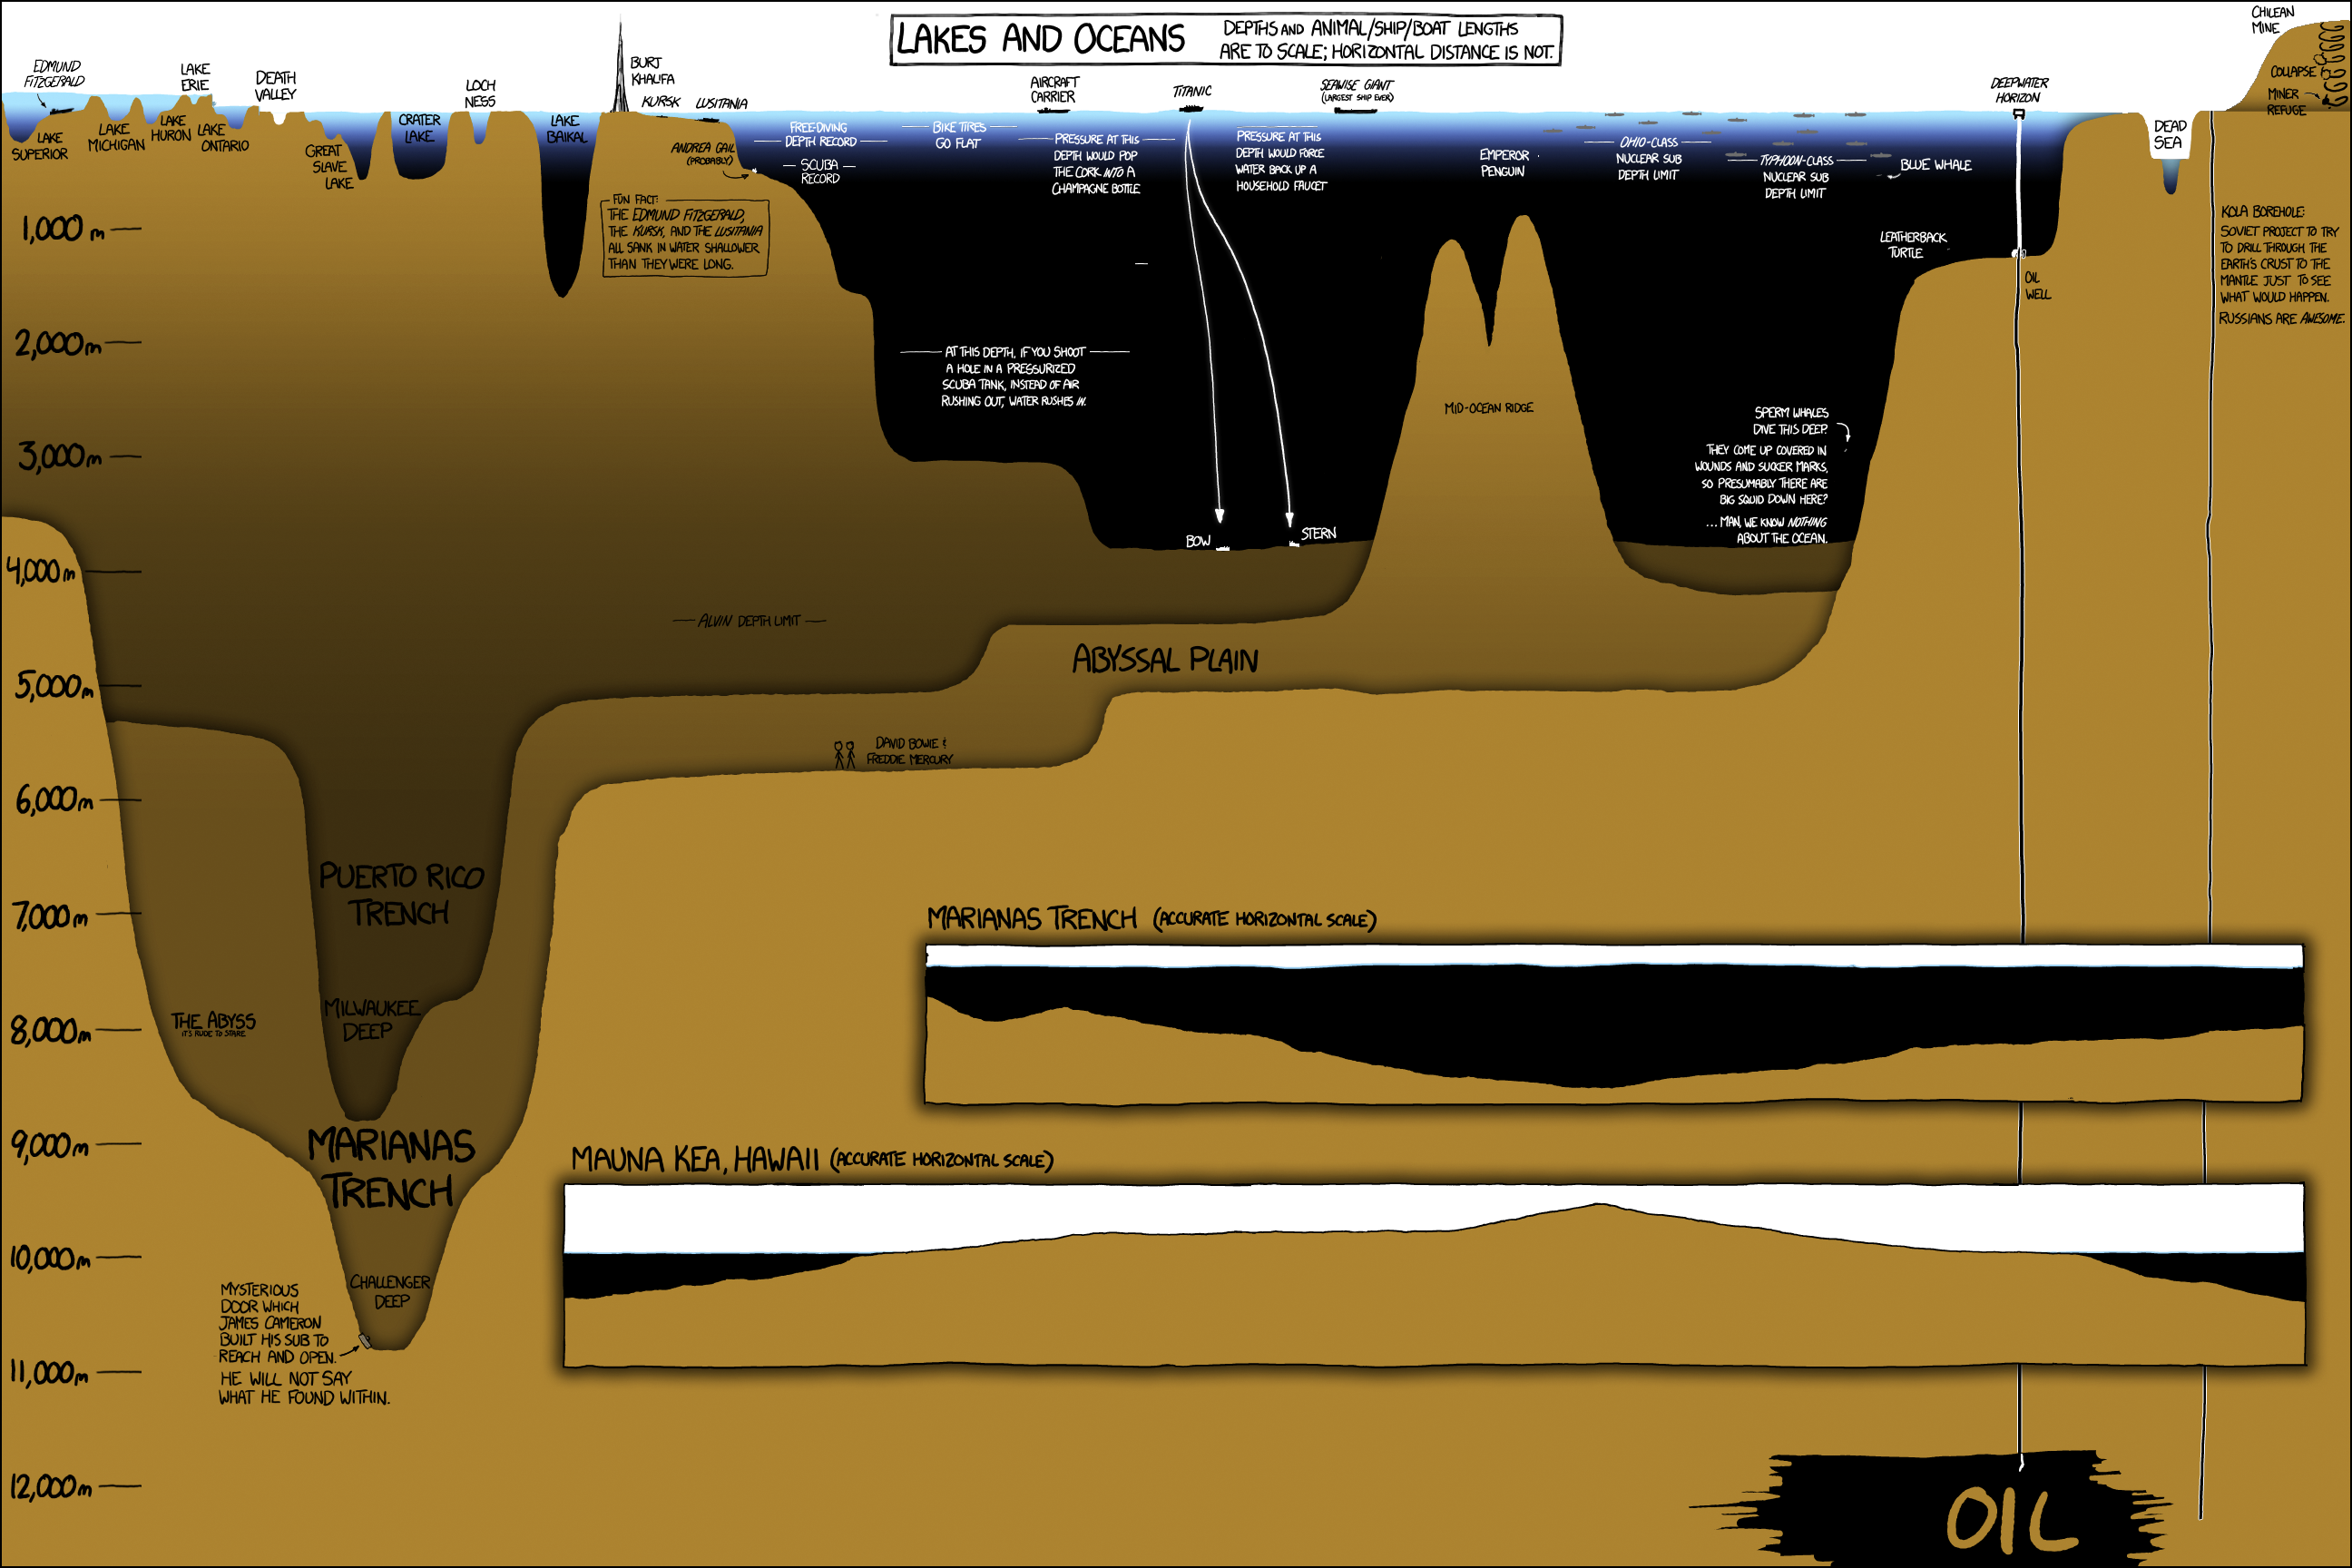
\includegraphics[scale=0.1, trim={0 0 55cm 0}, clip]{trench}};
    \begin{scope}[x={(image.south east)},y={(image.north west)}]
      \draw[red, thick, -stealth] (0.4, 0.75) -- +(120:0.2) node [black, pos=0, below] {\scriptsize Learning};
      \draw[red, thick, -stealth] (0.45, 0.05) -- +(100:0.08) node [black, pos=0, right] {\scriptsize Deep Learning};
    \end{scope}
  \end{tikzpicture}
    \end{figure}
  \end{column}
  \begin{column}{0.5\textwidth}
    \only<2->{TensorFlow is}
    \begin{itemize}
    \item<3-> An open source deep learning library
    \item<4-> Released by Google in November 2015
    \item<5-> Especially suited to:
      \begin{itemize}
        \item<6-> ``Large-scale machine learning on
        \item<6-> heterogenous distributed systems''
      \end{itemize}
    \end{itemize}
  \end{column}
\end{columns}
\end{frame}

%%% Local Variables:
%%% mode: latex
%%% TeX-master: "../presentation"
%%% End:
